\documentclass{report}

\usepackage[T1]{fontenc}
\usepackage{listings}
\usepackage{graphicx}
\usepackage{float}
\usepackage[a4paper, total={6in, 8in}]{geometry}
\usepackage{pdfpages}
\usepackage{comment}
\begin{document}

\title{Water-rocket-simulator code documentation}
\author{Manfred Gawlas}
\date{20.12.2023}

\maketitle

\tableofcontents

\chapter{Introduction}

%This document provides documentation for code of the Water Rocket Simulation as well as algorithms behind simulation. Program is writen in python using thinker and matplotlib libraries. It's main function is to provide a easy-to-use, efficient tool for designing rocket engines powered by pressurized gas and liquid. On top of that, optimalization part of program helps with understanding such motors.

This document serves as simple documentation for the Water Rocket Simulation program, detailing the underlying algorithms of the simulation. The program is implemented in Python, utilizing the Tkinter and Matplotlib libraries. Its primary purpose is to offer a easy-to-use and efficient tool for the design of rocket engines powered by pressurized gas and liquid. Additionally, the optimization component of the program may contributes to a deeper understanding of such propulsion systems for user.\\

Big thanks to Sebastian Król for helping with the whole project. Without him Kononowicz's prediction would come true, there would be nothing(nie było by niczego).  

\section{Code Overview}

The code consists of several parts, including:
\begin{itemize}
\item Variable declaration
\item Main simulation function
\item Optimalize function and simulation for optimalization loops
\item Plot functions
\item Save, load and export functions
\item Main thinker body
\end{itemize}

\section{Graphical user interface}
Program has a graphical interface which consits of 4 main regions. 
\begin{itemize}
\item Left plot - plot for data from single simulation
\item Left input table - list of entries for data needed to preform single simulation
\item Right plot - plot for data from optimalization
\item Right input table - list of entries for data to optimalize around
\end{itemize}

\chapter{Variables}

\section{Constants Declaration}
 
\begin{lstlisting}[language=Python]
delta_t = 0.0001
P_atm = float(1 * 101325)
\end{lstlisting}
The \texttt{delta\_t} variable represents the time step for the simulation. \texttt{P\_atm} is the atmospheric pressure.

\section{Simulation Output Data}

The code declares several arrays to store simulation output data such as time, height, thrust, mass, temperature, pressure, and volumes of water and air.

\begin{lstlisting}[language=Python]
array_time = []
array_h = []
array_Ft = []
array_mass = []
array_temperature = []
array_pressure = []
array_V_water = []
array_V_air = []
\end{lstlisting}

\section{Optimization Output Data}

Similar to simulation output data, there are arrays to store optimization output data.

\begin{lstlisting}[language=Python]
array_opt_x = []
array_opt_Ic = []
array_opt_tc = []
array_opt_delta_v = []
array_opt_Ist = []
opt_variable_name = ""
\end{lstlisting}

\section{Export Data}

Variables to store information about the rocket engine for export.

\begin{lstlisting}[language=Python]
engine_name = ""
engine_diameter = 0
engine_length = 0
engine_dry_mass = 0
engine_full_mass = 0
engine_manufacturer = ""
\end{lstlisting}

\chapter{Functions}

\section{Optimization Function}

\begin{lstlisting}[language=Python]
def optimize():
    # Function to optimize water rocket design
    ...
\end{lstlisting}
\begin{center}
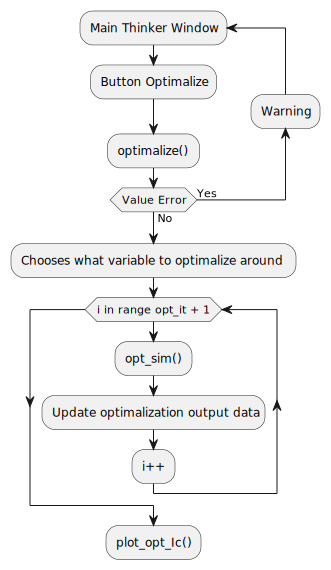
\includegraphics[scale=0.6]{optimalization}
\end{center}
\begin{comment}
@startuml
repeat :Main Thinker Window;
:Button Optimalize;
:optimalize();
backward :Warning;
repeat while (Value Error) is (Yes) not (No)
:Chooses what variable to optimalize around;
while(i in range opt_it + 1)
:opt_sim();
:Update optimalization output data;
:i++;
endwhile
:plot_opt_Ic();
@enduml
\end{comment}
The \texttt{optimize} function sets up and executes the optimization process based on user inputs and choosen variable.

\section{Simulation for optimalization}

\begin{lstlisting}[language=Python]
def opt_sim(k_const, Rs, water_density, P_ins, At, V_air, V_water, Roc_mass, T, 
rod_length, rod_inside_diameter):
    # Function to simulate water rocket flight for optimization
    ...
    return [Ic, total_time, Ic / (mass_propellant * 9.81), delta_v]
\end{lstlisting}

This function performs the numerical simulation of the water rocket's flight for optimization.


\section{Simulation Function}

\begin{lstlisting}[language=Python]
def simulate():
    # Function to simulate certain rocket motor
    ...
\end{lstlisting}
\begin{center}
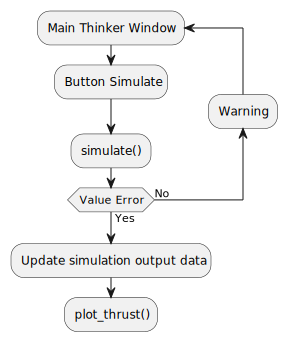
\includegraphics[scale=1]{simulate}
\end{center}
\begin{comment}
@startuml
repeat :Main Thinker Window;
:Button Simulate;
:simulate();
backward :Warning;
repeat while (Value Error) is (No) not (Yes)
:Update simulation output data;
:plot_thurst();
@enduml
\end{comment}
The \texttt{simulate} function executes simulation for a single data setup. It's responsible for left plot.


\section{Plotting Functions}

Functions to plot optimization results.

\begin{lstlisting}[language=Python]
def plot_opt_Ic():
    ...

def plot_opt_tc():
    ...

def plot_opt_Ist():
    ...

def plot_opt_delta_v():
    ...
\end{lstlisting}

These functions use the Matplotlib library to plot various optimization results. Optimalize and simulate functions have their coresponding plot functions.


\section{Save to File Function}

\begin{lstlisting}[language=Python]
def save_to_file(entry_text):
    # Function to save simulation parameters to a file
    ...
\end{lstlisting}

\section{Load from File Function}

\begin{lstlisting}[language=Python]
def load_from_file(entry_text):
    # Function to load simulation parameters from a file
    ...
\end{lstlisting}

\section{Export to File Function}

\begin{lstlisting}[language=Python]
def export_to_file():
    # Function to export simulation data to a .eng format
    ...
\end{lstlisting}
This function consits mainly of code for making additional window for export data that user needs to input.

\section{Save and Close Function}

\begin{lstlisting}[language=Python]
def save_and_close(entry_export_name, entry_export_diameter, entry_export_lenght, entry_export_man, window):
    # Function to save export parameters and close the export window
    ...
\end{lstlisting}

\section{Save to Export Function}

\begin{lstlisting}[language=Python]
def save_to_export():
    # Function to save exported data to a file
    ...
\end{lstlisting}

\chapter{Thinker GUI}
This part of code creates a Tkinter-based GUI application for a Water Rocket Simulator. Here's a summarised version of code:

\begin{lstlisting}[language=Python]
# Create the main Tkinter window
root = tk.Tk()
root.title("Water Rocket Simulator")

# Menu Bar
menubar = tk.Menu(root)
file_menu = tk.Menu(menubar, tearoff=0)
file_menu.add_command(label="Save", command=lambda: save_to_file(entry_0))
file_menu.add_command(label="Load", command=lambda: load_from_file(entry_0))
file_menu.add_command(label="Export as .eng", command=lambda: export_to_file())
menubar.add_cascade(label="File", menu=file_menu)
root.config(menu=menubar)

# Set the window size to full screen
screen_width = root.winfo_screenwidth()
screen_height = root.winfo_screenheight()
root.geometry(f"{screen_width}x{screen_height}")

# ... (Other setup code)

# LEFT
frame_simulate = ttk.Frame(root, padding="10")
# ... (Left frame setup)

# LEFT Plot
frame_plot_left = ttk.Frame(root, padding="10")
# ... (Matplotlib setup for left plot)

# RIGHT
frame_simulate_r = ttk.Frame(root, padding="10")
# ... (Right frame setup)

# RIGHT Plot
frame_plot_right = ttk.Frame(root, padding="10")
# ... (Matplotlib setup for right plot)

# Run the Tkinter event loop
root.mainloop()
\end{lstlisting}

Note: The code involves extensive GUI setup, including input fields, buttons, and plots using Tkinter and Matplotlib. It also incorporates error handling and dynamic updates based on user inputs.

\chapter{Simulation algorithm}
\section{Input variables}
Although the set of inputs for the user is easy to understand, this function takes another set of values as input, which can be calculated from user input. These are the same as below:

\begin{lstlisting}[language=Python]
def opt_sim(k_const, Rs, water_density, P_ins, At, V_air, V_water, Roc_mass, T,
rod_length, rod_inside_diameter):
\end{lstlisting}

\section{Structure}
The simulation consists of 5 while loops. The first two are responsible for the launch of the rod period, the third concerns the liquid expulsion phase, and the last two are responsible for the gas period.

\section{Lauch of rod phase}
If rod inside diameter is equal to 0 then we treat it as foregin volume inside chamber. Model is basicly an adibatic expansion of gas into volume left by pushed out rod. We calculate thrust simply as:
$$F = P_{ins} \cdot A_t$$
Rest is basicly numerical analysis for $\Delta t$.
$$v_e += a \cdot \Delta t \qquad a = \frac{F}{m_roc}$$
$$ \Delta V = A_t v_e \Delta t$$
Now we can calculate new volume of gas:
$$ V_{new} = V{old} + \Delta V$$
Using equation for adiabatic expansion:
$$ p V^k = const$$
$$ T = \frac{p V}{m Rs}$$
This concludes calculations for single time frame. All of this is in while loop, which can be expressed as:
\begin{lstlisting}[language=Python]
while( s < rod_lenght)
	s += s + ve*delta_t + a*delta_t*delta_t*0.5
	...
\end{lstlisting}
If rod inside diameter is higher then 0 the computational model is even simple, we assume that $$p=const, V=const, T=const$$
$$F=P_{ins}\cdot A_t$$

\section{Liquid expulsion phase}
During this phase we will again assume that thrust of motor is caused by adiabatic expansion of gas. For thrust we will use following equation:
$$F = \dot{m} v_e$$
Since velocities are relaltivly low we will use Bernoulies law which can be writen as:
$$ p_1 + \frac{\rho v_1^2}{2} = p_2 + \frac{\rho v_2^2}{2} $$
Since area of liquid facing gas inside is much greater then $A_t$ we assume that $v_1$ = 0. That gives negligible error.  From that we have:
$$ p_{ins} = p_{atm} + \frac{\rho v_e^2}{2} $$
$$v_e = \sqrt{2\frac{\Delta p}{\rho}}$$
$$\dot{m} = \rho\cdot A_t\cdot v_e$$
That gives:
$$ F = 2 A_t \Delta p$$
Now we calculate new values of V, P, T of gas.
$$\Delta V = A_t v_e \Delta t$$
$$pV^k = const$$
$$ T = \frac{p V}{m Rs}$$

\subsection*{Algorithm in steps}
\begin{enumerate}
\item $F_t = ...$
\item $v_e = ...$
\item $\Delta V =...$
\item $T = ...$
\item $m_{roc} -= \Delta V \cdot \rho_{wat}$
\item $ V_{air} = ... \qquad V_{wat} = ...$
\item $P_{ins} = ...$
\end{enumerate}


\section{Mach 1 gas expulsion phase}
We will treat this phase as a series of adiabatic expansions of gas. To calculate thurust we will use well known formula which I won't explain here.
$$F = \dot{m}v_e + A_t(p_{atm} - p_{ins})$$
Since this phase is for Mach 1 we can calculate $v_e$ in following manner:
$$v_e = M_e\cdot a_e = a_e = \sqrt{kRsT_t}$$
Now we use very cool formulas for Mach 1
$$T_t = \frac{2}{k+1}T^*$$
$$\rho_t = \left(\frac{2}{k+1}\right)^{\frac{1}{k-1}}\rho^*$$
$$\dot{m} = p^* A_t\left(\frac{2}{k+1}\right)^{\frac{k+1}{k-1}}\left(\frac{k}{RsT^*}\right)$$
Now for numerical solution:
$$\Delta m = \dot{m} \cdot \Delta t$$
$$\rho^*_{new} = \frac{m-\Delta m}{V}$$
$$p = \frac{mRsT}{V}$$
Now we rearange the adiabatic equation:
$$p_1v_1^k = p_2v_2^k$$ 
By substituting ideal gas equation and we get following equation for T:
$$T = \frac{p}{Rs}\left(\frac{V}{m_1}\right)^k\left(\frac{V}{m_1 - \Delta m}\right)^{1-k}$$
Now we compute it numericaly till we have Mach 1 on exit.\\\\
\subsection*{Algorithm in steps}
\begin{enumerate}
\item $T_t = ...$
\item $\dot{m} = ...$
\item $v_e = ...$
\item $P_t = ...\qquad F_t = ...$
\item $\Delta m = \dot{m}\cdot \Delta t \qquad m_{roc} = ...$
\item $T = ...\qquad P_{ins} = ...$
\end{enumerate}

\section{Sub Mach 1 gas expulsioin phase}
Calculations are similar but this time we have to calculate $M_e$. We assume $p_t = p_{atm}$.
$$M_e = \sqrt{\frac{2}{k-1}\left(\left(\frac{p_{ins}}{p_t}\right)^{\frac{k-1}{k}}-1\right)}$$
$$v_e = M_e\cdot a_e$$
Rest are just analogical equations for $M_e < 1$.\\\\

\subsection*{Algorithm in steps}
\begin{enumerate}
\item $M_e=...$
\item $T_t = ...$
\item $v_e = ...$
\item $\rho^* = ... \qquad \rho_t = ...$
\item $\dot{m} = ...$
\item $F_t = ...$
\item $\Delta m = \dot{m}\cdot \Delta t \qquad m_{roc} = ...$
\item $T = ...\qquad P_{ins} = ...$
\end{enumerate}
Now with the understanding of underlaying physics reader should have no problem understanding numerical computations behind simulation loops.

\begin{thebibliography}{9}
\bibitem{WaterRockets}
Michael de Podesta (2006) A guide to building and understanding the physics of Water Rockets, NPL

\bibitem{Seba}
Sebastian Król (2023) Rocketry formulas and derivations, PWr In Space
\end{thebibliography}


\end{document}